\documentclass[12pt,a4paper]{article}

% ─── Page Layout ───────────────────────────────────────────────────────────────
\usepackage[a4paper, margin=0.8in, headheight=14pt]{geometry}

% ─── Fonts (XeLaTeX) ───────────────────────────────────────────────────────────
\usepackage{fontspec}
\usepackage{unicode-math}
\setmainfont{TeX Gyre Pagella}
\setmonofont[Scale=0.88]{TeX Gyre Cursor}
\setmathfont{Latin Modern Math}

% ─── Packages ──────────────────────────────────────────────────────────────────
\usepackage{xcolor}
\usepackage{colortbl}
\usepackage{titlesec}
\usepackage{enumitem}
\usepackage{tabularx}
\usepackage{booktabs}
\usepackage{array}
\usepackage{amsmath}
\allowdisplaybreaks
\usepackage{tikz}
\usetikzlibrary{shapes.geometric, arrows.meta, positioning, calc, fit, decorations.pathreplacing, patterns}
\usepackage{tcolorbox}
\tcbuselibrary{skins, breakable}
\usepackage{hyperref}
\usepackage{fancyhdr}
\usepackage{graphicx}
\usepackage{microtype}
\hyphenpenalty=10000
\exhyphenpenalty=10000
\sloppy
\usepackage{caption}
\usepackage{setspace}
\usepackage{multirow}
\usepackage{tocloft}

% ─── Q&A helper ────────────────────────────────────────────────────────────────
\newcommand{\Q}[1]{\textbf{#1}\par\noindent\ignorespaces}

% ─── Colour Palette ────────────────────────────────────────────────────────────
\definecolor{myred}{RGB}{196,30,58}
\definecolor{mydark}{RGB}{30,30,50}
\definecolor{mygreen}{RGB}{14,120,80}
\definecolor{myteal}{RGB}{0,130,140}
\definecolor{myamber}{RGB}{180,100,0}
\definecolor{mypurple}{RGB}{100,30,160}
\definecolor{mygray}{RGB}{246,247,249}
\definecolor{mgframe}{RGB}{180,185,200}
\definecolor{watermark}{RGB}{145,150,170}
\definecolor{hdrred}{RGB}{250,232,235}
\definecolor{hdrgreen}{RGB}{220,244,233}
\definecolor{hdrteal}{RGB}{220,242,244}
\definecolor{hdramber}{RGB}{253,242,215}
\definecolor{hdrpurple}{RGB}{238,228,255}
\definecolor{hdrgray}{RGB}{238,240,245}
\definecolor{rowalt}{RGB}{250,251,253}

% ─── Section Formatting ────────────────────────────────────────────────────────
\titleformat{\section}
  {\large\bfseries\color{myred}}{\thesection.}{0.5em}{}
  [\vspace{1pt}{\color{myred}\rule{\linewidth}{0.8pt}}]
\titleformat{\subsection}
  {\normalsize\bfseries\color{myteal}}{\thesubsection}{0.5em}{}
\titlespacing*{\section}{0pt}{18pt}{7pt}
\titlespacing*{\subsection}{0pt}{11pt}{4pt}

% ─── Paragraph ─────────────────────────────────────────────────────────────────
\setlength{\parindent}{0pt}
\setlength{\parskip}{4pt}

% ─── TOC Styling ───────────────────────────────────────────────────────────────
\renewcommand{\cfttoctitlefont}{\large\bfseries\color{myred}}
\renewcommand{\cftaftertoctitle}{\par\noindent{\color{myred}\rule{\linewidth}{0.8pt}}}
\setlength{\cftbeforetoctitleskip}{0pt}
\setlength{\cftaftertoctitleskip}{6pt}
\renewcommand{\cftsecfont}{\normalsize\bfseries\color{mydark}}
\renewcommand{\cftsecpagefont}{\normalsize\bfseries\color{mydark}}
\renewcommand{\cftsecleader}{\cftdotfill{\cftdotsep}}
\setlength{\cftbeforesecskip}{7pt}
\renewcommand{\cftsubsecfont}{\small\color{mydark}}
\renewcommand{\cftsubsecpagefont}{\small\color{mydark}}
\setlength{\cftbeforesubsecskip}{3pt}
\setlength{\cftsubsecindent}{1.4em}

% ─── Table helpers ─────────────────────────────────────────────────────────────
\renewcommand{\arraystretch}{1.45}
\setlength{\tabcolsep}{6pt}
\arrayrulecolor{mydark}
\newcolumntype{B}[1]{>{\small\bfseries\raggedright\arraybackslash}m{#1}}
\newcolumntype{Y}{>{\small\raggedright\arraybackslash}X}
\renewcommand{\tabularxcolumn}[1]{m{#1}}

% ─── Header / Footer ───────────────────────────────────────────────────────────
\pagestyle{fancy}
\fancyhf{}
\fancyhead[L]{\small\color{myred}\textbf{EC302}\;\color{mydark}--- Digital System Design}
\fancyhead[R]{\small\color{myteal}\textbf{Module 1 Notes}}
\fancyfoot[C]{\small\color{mydark}\thepage}
\fancyfoot[R]{\small\color{watermark}\textit{\copyright\ Biraj}}
\renewcommand{\headrulewidth}{0.5pt}
\renewcommand{\footrulewidth}{0.3pt}

% ─── Hyperref ──────────────────────────────────────────────────────────────────
\hypersetup{
  colorlinks=true, linkcolor=myteal, urlcolor=myteal,
  pdfauthor={Biraj Sarkar (CGEC)},
  pdftitle={EC302 --- Module 1 Notes: Number Systems, Boolean Algebra, and Combinational Logic}
}

% ─── tcolorbox styles ──────────────────────────────────────────────────────────
\tcbset{
  tikzbox/.style={
    colback=mygray, colframe=mgframe, boxrule=0.6pt, arc=4pt,
    left=8pt, right=8pt, top=6pt, bottom=6pt,
    colbacktitle=mgframe, coltitle=mydark,
    fonttitle=\small\bfseries
  },
  defbox/.style={
    colback=hdrgreen, colframe=mygreen, boxrule=0.8pt, arc=4pt,
    left=9pt, right=9pt, top=6pt, bottom=6pt,
    colbacktitle=mygreen, coltitle=white,
    fonttitle=\small\bfseries
  },
  formulabox/.style={
    colback=hdrteal, colframe=myteal, boxrule=0.8pt, arc=4pt,
    left=9pt, right=9pt, top=6pt, bottom=6pt,
    colbacktitle=myteal, coltitle=white,
    fonttitle=\small\bfseries
  },
  examplebox/.style={
    colback=hdramber, colframe=myamber, boxrule=0.8pt, arc=4pt,
    left=9pt, right=9pt, top=6pt, bottom=6pt,
    colbacktitle=myamber, coltitle=white,
    fonttitle=\small\bfseries
  },
  masonbox/.style={
    colback=hdrpurple, colframe=mypurple, boxrule=0.8pt, arc=4pt,
    left=9pt, right=9pt, top=6pt, bottom=6pt,
    colbacktitle=mypurple, coltitle=white,
    fonttitle=\small\bfseries
  },
  exambox/.style={
    colback=hdrpurple, colframe=mypurple, boxrule=1pt, arc=5pt,
    left=10pt, right=10pt, top=8pt, bottom=8pt,
    colbacktitle=mypurple, coltitle=white,
    fonttitle=\bfseries,
    breakable, title after break={\textbf{Frequently Asked / Viva Questions (contd.)}}
  }
}

\tcbset{breakable}
\tcbset{after={\color{black}}}

% ─── TikZ styles ───────────────────────────────────────────────────────────────
\tikzset{
  block/.style={rectangle, draw=myteal, fill=hdrteal,
    text width=2.4cm, align=center, minimum height=0.95cm,
    font=\small, rounded corners=3pt, line width=0.7pt},
  redblock/.style={rectangle, draw=myred, fill=hdrred,
    text width=2.4cm, align=center, minimum height=0.95cm,
    font=\small, rounded corners=3pt, line width=0.7pt},
  greenblock/.style={rectangle, draw=mygreen, fill=hdrgreen,
    text width=2.4cm, align=center, minimum height=0.95cm,
    font=\small, rounded corners=3pt, line width=0.7pt},
  sum/.style={circle, draw=myred, fill=hdrred,
    inner sep=2pt, minimum size=0.6cm, line width=0.7pt},
  flowarrow/.style={-Stealth, thick, color=mydark},
  sblock/.style={rectangle, draw=myteal, fill=hdrteal,
    text width=1.5cm, align=center, minimum height=0.75cm,
    font=\scriptsize, rounded corners=2pt, line width=0.6pt}
}

\begin{document}

\begin{center}
  {\LARGE\bfseries\color{myred} EC302 --- Digital System Design}\\[5pt]
  {\normalsize\color{mydark} Semester III \quad$\bullet$\quad 3L:0T:0P \quad$\bullet$\quad 3 Credits}\\[3pt]
  {\normalsize\color{myteal}\textbf{Module 1 Exam Notes: Number Systems, Boolean Algebra \& Combinational Logic}}\\[3pt]
  {\small\color{mydark} CGEC \;$|$\; B.Tech ECE (2023--27) \;$|$\; \textit{Biraj Sarkar}}
\end{center}
\vspace{2pt}
\noindent{\color{myred}\rule{\linewidth}{1.5pt}}
\vspace{2pt}

\hypersetup{linkcolor=mydark}
\tableofcontents
\hypersetup{linkcolor=myteal}
\newpage

% ===============================================================================
\section{Number Systems and Binary Arithmetic}
% ===============================================================================

Digital systems process discrete electrical signals representing numerical data in positional number systems. A number $N$ in a base (radix) $r$ is represented as:
\begin{equation}
  (N)_r = \sum_{i=-m}^{n-1} d_i \cdot r^i = d_{n-1} r^{n-1} + \dots + d_1 r^1 + d_0 r^0 + d_{-1} r^{-1} + \dots + d_{-m} r^{-m}
\end{equation}
where $0 \le d_i \le (r-1)$, $n$ is the number of integer digits, and $m$ is the number of fractional digits.

\subsection{Radix Conversions}
\begin{itemize}[leftmargin=*, itemsep=3pt]
  \item \textbf{Base-$r$ to Decimal:} Expand the number into polynomials of powers of $r$.
  \item \textbf{Decimal to Base-$r$:} Divide the integer portion successively by $r$ (collecting remainders from LSB to MSB); multiply the fractional portion successively by $r$ (collecting integer carries from MSB to LSB).
  \item \textbf{Binary, Octal, and Hexadecimal Conversions:} Because $8 = 2^3$ and $16 = 2^4$, conversion between binary and octal requires grouping bits into groups of 3; conversion between binary and hexadecimal requires grouping bits into groups of 4.
\end{itemize}

\subsection{Representation of Signed Numbers}
In an $n$-bit binary system, unsigned numbers range from $0$ to $2^n - 1$. Signed numbers dedicate the most significant bit (MSB) as the sign bit: $\text{MSB} = 0 \implies \text{Positive}$, $\text{MSB} = 1 \implies \text{Negative}$.

\begin{tcolorbox}[defbox, title={\textbf{Three Signed Number Representations ($n$-bit)}}]
\begin{enumerate}[label=\arabic*., leftmargin=*]
  \item \textbf{Signed Magnitude:}
    $\text{Magnitude}$ is stored in the lower $(n-1)$ bits.
    \begin{equation}
      \text{Range: } -(2^{n-1}-1) \le N \le +(2^{n-1}-1)
    \end{equation}
    Drawback: Two distinct representations for zero ($+0 = 0000_2$, $-0 = 1000_2$), complicating ALU hardware.
  \item \textbf{1's Complement:}
    Negative numbers are formed by bitwise inverting all $n$ bits of the positive magnitude.
    \begin{equation}
      \text{Range: } -(2^{n-1}-1) \le N \le +(2^{n-1}-1)
    \end{equation}
    Drawback: Dual representation for zero ($+0 = 0000_2$, $-0 = 1111_2$); requires an end-around carry addition.
  \item \textbf{2's Complement (Universal Standard):}
    Negative numbers are formed by adding $1$ to the 1's complement ($N_{2's} = 2^n - |N|$).
    \begin{equation}
      \text{Range: } -2^{n-1} \le N \le +(2^{n-1}-1)
    \end{equation}
    Advantages: Single, unique representation for zero ($0000_2$); arithmetic subtraction is performed using standard binary addition without end-around carry; extra negative value can be represented.
\end{enumerate}
\end{tcolorbox}

\subsection{2's Complement Arithmetic and Overflow Detection}
To compute $A - B$, the digital processor computes $A + (\text{2's complement of } B)$. An end-carry produced out of the MSB is simply discarded.

\begin{tcolorbox}[formulabox, title={\textbf{Arithmetic Overflow Rule in 2's Complement}}]
Overflow occurs when an addition of two numbers with identical signs produces an invalid result with an opposite sign. Overflow cannot occur when adding numbers with opposite signs.
\begin{equation}
  V = C_n \oplus C_{n-1}
\end{equation}
where $C_n$ is the carry out of the sign bit (MSB), and $C_{n-1}$ is the carry into the sign bit. If $V = 1$, arithmetic overflow has occurred, indicating the result exceeds the allowable $n$-bit range.
\end{tcolorbox}

% ===============================================================================
\section{Boolean Algebra and Logic Simplification}
% ===============================================================================

Boolean algebra is an algebraic structure defined on a set of elements $B = \{0, 1\}$ with two binary operators ($+$ OR, $\cdot$ AND) and one unary operator ($'$ NOT).

\subsection{Fundamental Laws of Boolean Algebra}
\par\vspace{6pt}\noindent
\begingroup
\setlength{\tabcolsep}{4pt}
\setlength{\extrarowheight}{2.5pt}
\renewcommand{\arraystretch}{1.35}
\begin{tabularx}{\linewidth}{|B{3.4cm}|Y|Y|}
\hline
\textbf{Law / Property} & \textbf{AND Form} & \textbf{OR Form} \\
\hline
Identity Law & $A \cdot 1 = A$ & $A + 0 = A$ \\
\hline
Null (Annulment) Law & $A \cdot 0 = 0$ & $A + 1 = 1$ \\
\hline
Idempotent Law & $A \cdot A = A$ & $A + A = A$ \\
\hline
Complement Law & $A \cdot A' = 0$ & $A + A' = 1$ \\
\hline
Involution (Double Negation) & \multicolumn{2}{c|}{$(A')' = A$} \\
\hline
\end{tabularx}
\endgroup

\par\vspace{6pt}\noindent
\begingroup
\setlength{\tabcolsep}{4pt}
\setlength{\extrarowheight}{2.5pt}
\renewcommand{\arraystretch}{1.35}
\begin{tabularx}{\linewidth}{|B{3.4cm}|Y|Y|}
\hline
\textbf{Law / Property (contd.)} & \textbf{AND Form} & \textbf{OR Form} \\
\hline
Commutative Law & $A \cdot B = B \cdot A$ & $A + B = B + A$ \\
\hline
Associative Law & $A \cdot (B \cdot C) = (A \cdot B) \cdot C$ & $A + (B + C) = (A + B) + C$ \\
\hline
Distributive Law & $A \cdot (B + C) = A \cdot B + A \cdot C$ & $A + (B \cdot C) = (A + B) \cdot (A + C)$ \\
\hline
Absorption Law & $A \cdot (A + B) = A$ & $A + A \cdot B = A$ \\
\hline
Consensus Theorem & $(A+B)(A'+C)(B+C) = (A+B)(A'+C)$ & $AB + A'C + BC = AB + A'C$ \\
\hline
\end{tabularx}
\endgroup

\subsection{De Morgan's Theorems and the Principle of Duality}
\begin{tcolorbox}[formulabox, title={\textbf{De Morgan's Theorems}}]
\begin{align}
  \overline{A \cdot B \cdot C \dots} &= \overline{A} + \overline{B} + \overline{C} + \dots \quad \text{(NAND gate is equivalent to a Bubbled-OR gate)} \\
  \overline{A + B + C + \dots} &= \overline{A} \cdot \overline{B} \cdot \overline{C} \dots \quad \text{(NOR gate is equivalent to a Bubbled-AND gate)}
\end{align}
\end{tcolorbox}

\textbf{Principle of Duality:} Any true Boolean identity remains valid if:
\begin{enumerate}[label=\alph*., leftmargin=*]
  \item Every $+$ (OR) operator is replaced with $\cdot$ (AND), and vice versa.
  \item Every $0$ is replaced with $1$, and vice versa.
  \item Literal variables remain uncomplemented.
\end{enumerate}

\subsection{Canonical and Standard Forms}
\begin{itemize}[leftmargin=*, itemsep=3pt]
  \item \textbf{Minterm ($m_i$):} A product (AND) of all $n$ literals in which each variable appears exactly once in true or complemented form. A minterm equals $1$ for exactly one input combination.
  \item \textbf{Maxterm ($M_i$):} A sum (OR) of all $n$ literals in which each variable appears exactly once. A maxterm equals $0$ for exactly one input combination.
  \item \textbf{Complementary Duality:}
  \begin{equation}
    M_i = \overline{m_i}, \qquad f(A, B, C) = \sum m(1, 4, 6, 7) = \prod M(0, 2, 3, 5)
  \end{equation}
  \item \textbf{Sum of Products (SOP):} Canonical form summing all minterms where the function is $1$.
  \item \textbf{Product of Sums (POS):} Canonical form multiplying all maxterms where the function is $0$.
\end{itemize}

% ===============================================================================
\section{Karnaugh Map (K-Map) Simplification}
% ===============================================================================

The Karnaugh Map is a graphical truth-table layout where adjacent squares differ in only a single bit position (Gray code ordering: $00, 01, 11, 10$).

\subsection{Grouping Principles and Implicants}
\begin{enumerate}[label=\arabic*., leftmargin=*]
  \item Adjacent squares containing $1$s are combined into groups of sizes that are powers of two ($1, 2, 4, 8, 16$).
  \item Grouping $2^k$ adjacent cells eliminates $k$ variables.
  \item \textbf{Implicant:} Any single minterm or combination of minterms that can be grouped.
  \item \textbf{Prime Implicant (PI):} A rectangle of $1$s that cannot be merged with any larger group.
  \item \textbf{Essential Prime Implicant (EPI):} A prime implicant that covers at least one minterm ($1$) not covered by any other prime implicant. All EPIs must be included in the minimal Boolean expression.
  \item \textbf{Don't Care Conditions ($d$ or $X$):} Input combinations that can never occur in practice. They can be treated as $1$s if they help enlarge a group, or as $0$s if they do not.
\end{enumerate}

\begin{tcolorbox}[tikzbox, title={4-Variable Karnaugh Map Cell Topology and Adjacency Structure}]
\centering
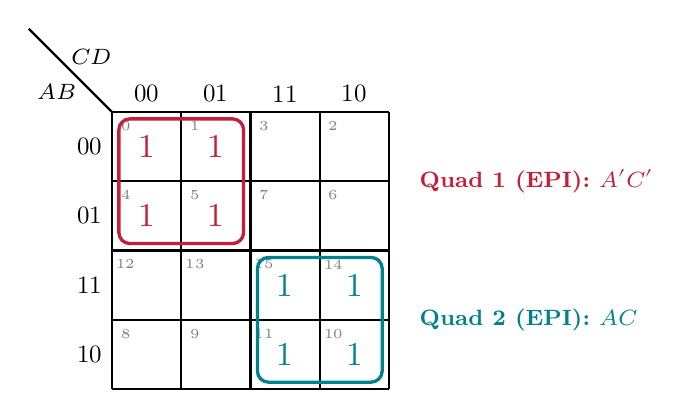
\begin{tikzpicture}[scale=0.88]
  % Grid
  \draw[thick] (0,0) grid (4,4);
  \draw[thick] (0,4) -- (-1.2, 5.2);
  \node[font=\footnotesize\bfseries] at (-0.8, 4.3) {$AB$};
  \node[font=\footnotesize\bfseries] at (-0.3, 4.8) {$CD$};

  % Column headers (CD)
  \node[above, font=\small] at (0.5, 4) {$00$};
  \node[above, font=\small] at (1.5, 4) {$01$};
  \node[above, font=\small] at (2.5, 4) {$11$};
  \node[above, font=\small] at (3.5, 4) {$10$};

  % Row headers (AB)
  \node[left, font=\small] at (0, 3.5) {$00$};
  \node[left, font=\small] at (0, 2.5) {$01$};
  \node[left, font=\small] at (0, 1.5) {$11$};
  \node[left, font=\small] at (0, 0.5) {$10$};

  % Minterm indices (gray)
  \node[font=\tiny\color{gray}] at (0.2, 3.8) {$0$};
  \node[font=\tiny\color{gray}] at (1.2, 3.8) {$1$};
  \node[font=\tiny\color{gray}] at (2.2, 3.8) {$3$};
  \node[font=\tiny\color{gray}] at (3.2, 3.8) {$2$};

  \node[font=\tiny\color{gray}] at (0.2, 2.8) {$4$};
  \node[font=\tiny\color{gray}] at (1.2, 2.8) {$5$};
  \node[font=\tiny\color{gray}] at (2.2, 2.8) {$7$};
  \node[font=\tiny\color{gray}] at (3.2, 2.8) {$6$};

  \node[font=\tiny\color{gray}] at (0.2, 1.8) {$12$};
  \node[font=\tiny\color{gray}] at (1.2, 1.8) {$13$};
  \node[font=\tiny\color{gray}] at (2.2, 1.8) {$15$};
  \node[font=\tiny\color{gray}] at (3.2, 1.8) {$14$};

  \node[font=\tiny\color{gray}] at (0.2, 0.8) {$8$};
  \node[font=\tiny\color{gray}] at (1.2, 0.8) {$9$};
  \node[font=\tiny\color{gray}] at (2.2, 0.8) {$11$};
  \node[font=\tiny\color{gray}] at (3.2, 0.8) {$10$};

  % Example 1s
  \node[font=\large\bfseries\color{myred}] at (0.5, 3.5) {$1$};
  \node[font=\large\bfseries\color{myred}] at (1.5, 3.5) {$1$};
  \node[font=\large\bfseries\color{myred}] at (0.5, 2.5) {$1$};
  \node[font=\large\bfseries\color{myred}] at (1.5, 2.5) {$1$};

  \node[font=\large\bfseries\color{myteal}] at (2.5, 1.5) {$1$};
  \node[font=\large\bfseries\color{myteal}] at (3.5, 1.5) {$1$};
  \node[font=\large\bfseries\color{myteal}] at (2.5, 0.5) {$1$};
  \node[font=\large\bfseries\color{myteal}] at (3.5, 0.5) {$1$};

  % Grouping boxes
  \draw[very thick, rounded corners=4pt, color=myred] (0.1, 2.1) rectangle (1.9, 3.9);
  \node[right, font=\footnotesize\bfseries\color{myred}] at (4.3, 3.0) {Quad 1 (EPI): $A' C'$};

  \draw[very thick, rounded corners=4pt, color=myteal] (2.1, 0.1) rectangle (3.9, 1.9);
  \node[right, font=\footnotesize\bfseries\color{myteal}] at (4.3, 1.0) {Quad 2 (EPI): $A C$};
\end{tikzpicture}
\end{tcolorbox}

\subsection{Static Hazards in Combinational Logic}
A \textbf{static hazard} is a transient unwanted glitch ($0 \to 1 \to 0$ for static-0 or $1 \to 0 \to 1$ for static-1) occurring at the output due to unequal propagation delays along converging signal paths.
\begin{itemize}[leftmargin=*, itemsep=3pt]
  \item \textbf{Cause:} A single variable changes state and transitions between two adjacent K-map prime implicant loops without an overlapping product term.
  \item \textbf{Elimination:} Add redundant consensus prime implicants to bridge adjacent loops in the K-map.
\end{itemize}

% ===============================================================================
\section{Binary Codes and Code Converters}
% ===============================================================================

Digital systems employ specialized binary codes tailored for arithmetic, display, communication, and mechanical position sensing:

\subsection{Standard Binary Codes}
\begin{itemize}[leftmargin=*, itemsep=3pt]
  \item \textbf{BCD (Binary Coded Decimal / 8421):} Each decimal digit ($0\text{--}9$) is encoded as a 4-bit binary group ($0000$ to $1001$). The six combinations $1010_2$ to $1111_2$ are invalid.
  \item \textbf{Excess-3 Code:} Unweighted, self-complementing code formed by adding $0011_2$ ($+3$) to the 8421 BCD code. The 1's complement of an Excess-3 number represents the 9's complement of its decimal equivalent.
  \item \textbf{Gray Code (Reflected Binary Unit-Distance Code):} Successive code words differ in only a single bit position ($\Delta = 1$), eliminating spurious switching errors in optical shaft encoders.
\end{itemize}

\subsection{Binary to Gray and Gray to Binary Code Conversion}
\begin{tcolorbox}[formulabox, title={\textbf{Code Conversion Logic}}]
Binary to Gray conversion ($B = b_{n-1} \dots b_0 \to G = g_{n-1} \dots g_0$):
\begin{equation}
  g_{n-1} = b_{n-1}, \qquad g_i = b_{i+1} \oplus b_i \quad (\text{for } i = 0, 1, \dots, n-2)
\end{equation}
Gray to Binary conversion ($G = g_{n-1} \dots g_0 \to B = b_{n-1} \dots b_0$):
\begin{equation}
  b_{n-1} = g_{n-1}, \qquad b_i = b_{i+1} \oplus g_i \quad (\text{for } i = 0, 1, \dots, n-2)
\end{equation}
\end{tcolorbox}

% ===============================================================================
\section{Combinational Arithmetic Circuits}
% ===============================================================================

\subsection{Half Adder, Full Adder, and Subtractors}
\par\vspace{6pt}\noindent
\begingroup
\setlength{\tabcolsep}{4pt}
\setlength{\extrarowheight}{3pt}
\renewcommand{\arraystretch}{1.35}
\begin{tabularx}{\linewidth}{|B{2.8cm}|Y|Y|}
\hline
\textbf{Circuit} & \textbf{Boolean Sum / Difference ($S, D$)} & \textbf{Carry / Borrow ($C, B$)} \\
\hline
Half Adder (HA) & $S = A \oplus B$ & $C = A \cdot B$ \\
\hline
Half Subtractor (HS) & $D = A \oplus B$ & $B_{\text{out}} = A' \cdot B$ \\
\hline
Full Adder (FA) & $S = A \oplus B \oplus C_{\text{in}}$ & $C_{\text{out}} = A B + (A \oplus B) C_{\text{in}} = A B + B C_{\text{in}} + A C_{\text{in}}$ \\
\hline
Full Subtractor (FS) & $D = A \oplus B \oplus B_{\text{in}}$ & $B_{\text{out}} = A' B + (A \oplus B)' B_{\text{in}} = A' B + A' B_{\text{in}} + B B_{\text{in}}$ \\
\hline
\end{tabularx}
\endgroup

\subsection{Ripple Carry Adder vs. Carry Lookahead Adder (CLA)}
An $n$-bit \textbf{Ripple Carry Adder (RCA)} cascades $n$ Full Adders. The carry out of stage $i$ ripples to the carry input of stage $i+1$. Total worst-case propagation delay is linear:
\begin{equation}
  t_{\text{RCA}} = 2 t_{\text{gate}} + (n-1) 2 t_{\text{gate}} = 2 n \, t_{\text{gate}}
\end{equation}
To eliminate rippling delay, the \textbf{Carry Lookahead Adder (CLA)} precomputes all stage carries in parallel using Carry Generate ($G_i$) and Carry Propagate ($P_i$) functions:
\begin{equation}
  G_i = A_i \cdot B_i, \qquad P_i = A_i \oplus B_i
\end{equation}
Expanding the stage carry expressions recursively:
\begin{align}
  C_1 &= G_0 + P_0 C_0 \\
  C_2 &= G_1 + P_1 C_1 = G_1 + P_1 G_0 + P_1 P_0 C_0 \\
  C_3 &= G_2 + P_2 G_1 + P_2 P_1 G_0 + P_2 P_1 P_0 C_0 \\
  C_4 &= G_3 + P_3 G_2 + P_3 P_2 G_1 + P_3 P_2 P_1 G_0 + P_3 P_2 P_1 P_0 C_0
\end{align}

\begin{tcolorbox}[tikzbox, title={Carry Lookahead Generator Architecture (4-bit CLA)}]
\centering
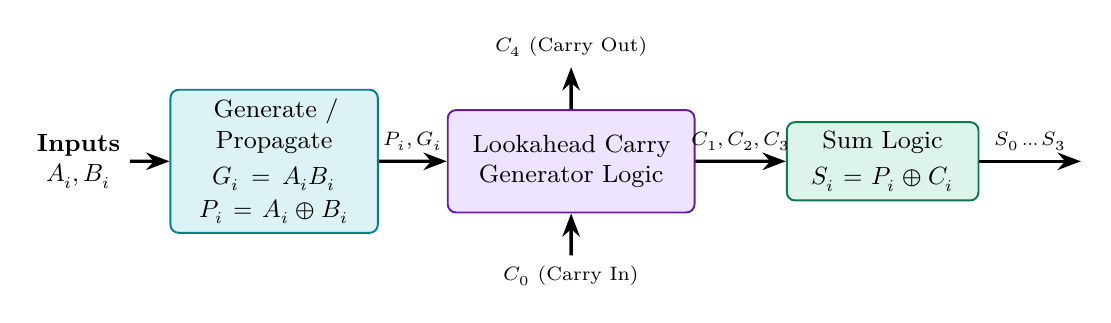
\begin{tikzpicture}[scale=0.92]
  % Inputs
  \node[font=\small\bfseries, align=center] (in) at (0.6, 2.5) {Inputs\\$A_i, B_i$};
  
  % Block 1: Generate / Propagate
  \node[block, fill=hdrteal, draw=myteal, text width=2.4cm] (gp) at (3.3, 2.5) {Generate / Propagate\\[2pt]$G_i = A_i B_i$\\[1pt]$P_i = A_i \oplus B_i$};

  % Block 2: Lookahead Carry Generator
  \node[block, fill=hdrpurple, draw=mypurple, text width=2.9cm, minimum height=1.3cm] (clg) at (7.4, 2.5) {Lookahead Carry\\Generator Logic};

  % Block 3: Sum Logic
  \node[block, fill=hdrgreen, draw=mygreen, text width=2.2cm] (sum) at (11.7, 2.5) {Sum Logic\\[2pt]$S_i = P_i \oplus C_i$};

  % Connecting Arrows & Labels
  \draw[-Stealth, very thick] (in) -- (gp);
  \draw[-Stealth, very thick] (gp) -- (clg) node[midway, above, font=\scriptsize] {$P_i, G_i$};
  \draw[-Stealth, very thick] (clg) -- (sum) node[midway, above, font=\scriptsize] {$C_1, C_2, C_3$};
  \draw[-Stealth, very thick] (7.4, 1.2) node[below, font=\scriptsize] {$C_0 \text{ (Carry In)}$} -- (clg.south);
  \draw[-Stealth, very thick] (clg.north) -- (7.4, 3.8) node[above, font=\scriptsize] {$C_4 \text{ (Carry Out)}$};
  \draw[-Stealth, very thick] (sum.east) -- ++(1.4, 0) node[midway, above, font=\scriptsize] {$S_0 \dots S_3$};
\end{tikzpicture}
\end{tcolorbox}

\par\vspace{4pt}\noindent
\textbf{Delay Comparison:} All carries $C_1, \dots, C_4$ are generated in only $2 t_{\text{gate}}$ delays, and the final sums in $4 t_{\text{gate}}$ delays, completely independent of word length $n$.

\subsection{BCD Adder}
Adding two 4-bit BCD digits produces a sum $S_3 S_2 S_1 S_0$ and carry $K$. When the sum exceeds $9$ ($1001_2$) or a carry $K=1$ is generated, the result is an invalid BCD digit. Correction is achieved by adding $6$ ($0110_2$):
\begin{equation}
  \text{Correction Flag } C_{\text{out}} = K + S_3 S_2 + S_3 S_1
\end{equation}

% ===============================================================================
\section{MSI Combinational Logic Devices}
% ===============================================================================

\subsection{Magnitude Comparators}
A magnitude comparator compares two $n$-bit binary numbers $A = a_{n-1} \dots a_0$ and $B = b_{n-1} \dots b_0$ and asserts one of three output lines: $A > B$, $A = B$, or $A < B$.
\begin{itemize}[leftmargin=*, itemsep=3pt]
  \item Equality condition: $A = B \implies x_i = (a_i \oplus b_i)'$ for all $i$, so $(A=B) = x_{n-1} x_{n-2} \dots x_0$.
  \item Greater-than condition:
  \begin{equation}
    (A > B) = a_{n-1} b_{n-1}' + x_{n-1} a_{n-2} b_{n-2}' + \dots + x_{n-1} \dots x_1 a_0 b_0'
  \end{equation}
  \item IC 7485 is a 4-bit magnitude comparator equipped with cascading inputs ($I_{A>B}, I_{A=B}, I_{A<B}$) enabling expansion to compare 8-bit, 16-bit, or larger words.
\end{itemize}

\subsection{Multiplexers (Data Selectors)}
A multiplexer routes one of $2^n$ data input channels to a single output line under the control of $n$ selection lines:
\begin{equation}
  Y = \sum_{k=0}^{2^n-1} m_k \cdot D_k
\end{equation}
where $m_k$ is the minterm formed by the $n$ select lines $S_{n-1} \dots S_0$.
\begin{itemize}[leftmargin=*, itemsep=3pt]
  \item \textbf{Universal Logic Implementation:} Any Boolean function of $n$ variables can be implemented directly using a $2^{n-1}$-to-1 MUX by connecting $(n-1)$ variables to select lines and using the remaining variable ($0, 1, X, X'$) on the data inputs.
\end{itemize}

\subsection{Encoders and Decoders}
\begin{itemize}[leftmargin=*, itemsep=3pt]
  \item \textbf{Decoders ($n$-to-$2^n$):} Converts an $n$-bit binary input into one of $2^n$ active output lines (minterm generator). IC 74138 is a standard 3-to-8 decoder with active-low outputs.
  \item \textbf{Priority Encoders ($2^n$-to-$n$):} If two or more inputs are simultaneously asserted, the encoder generates the binary code corresponding to the input with the highest assigned priority (e.g., IC 74148 8-to-3 priority encoder).
\end{itemize}

\subsection{Barrel Shifters and Arithmetic Logic Units (ALUs)}
\begin{itemize}[leftmargin=*, itemsep=3pt]
  \item \textbf{Barrel Shifter:} A specialized digital crossbar circuit constructed from multiplexer arrays capable of shifting or rotating an $n$-bit data word by an arbitrary number of bit positions ($0$ to $n-1$) in a \textbf{single clock cycle}, avoiding sequential shift register clock cycles.
  \item \textbf{Arithmetic Logic Unit (IC 74181):} A 4-bit parallel multifunction processor element. Under the command of 4 function select inputs ($S_3 S_2 S_1 S_0$) and a mode control bit $M$ ($M=1 \implies$ Logic functions; $M=0 \implies$ Arithmetic functions with carry lookahead), it can perform all 16 logic operations and 16 arithmetic operations.
\end{itemize}

\newpage
% ===============================================================================
% MANDATORY QUICK REVISION PAGE
% ===============================================================================
\begin{center}
  {\large\bfseries\color{myred} Quick Revision --- Module 1}\\[3pt]
  {\small\color{mydark} Number Systems, Boolean Algebra \& Combinational Logic $|$ EC302}
\end{center}
\noindent{\color{myred}\rule{\linewidth}{1.2pt}}
\vspace{4pt}

\begin{tcolorbox}[formulabox, title={\textbf{Key Formulas and Identities at a Glance}}]
\renewcommand{\arraystretch}{1.35}
\begin{tabularx}{\linewidth}{B{5.2cm} X}
Signed 2's Complement Range & $-2^{n-1} \le N \le 2^{n-1}-1$ \\[4pt]
2's Complement Overflow Condition & $V = C_n \oplus C_{n-1}$ \\[4pt]
De Morgan's Laws & $\overline{A \cdot B} = \overline{A} + \overline{B}, \quad \overline{A + B} = \overline{A} \cdot \overline{B}$ \\[4pt]
Binary-to-Gray Conversion & $g_{n-1} = b_{n-1}, \quad g_i = b_{i+1} \oplus b_i$ \\[4pt]
Full Adder Sum \& Carry & $S = A \oplus B \oplus C_{\text{in}}, \quad C_{\text{out}} = AB + (A \oplus B)C_{\text{in}}$ \\[4pt]
CLA Generate \& Propagate & $G_i = A_i B_i, \quad P_i = A_i \oplus B_i, \quad C_{i+1} = G_i + P_i C_i$ \\[4pt]
BCD Adder Correction Flag & $C_{\text{out}} = K + S_3 S_2 + S_3 S_1$ \\[4pt]
Multiplexer Output Equation & $Y = \sum_{k=0}^{2^n-1} m_k D_k$ \\[4pt]
\end{tabularx}
\end{tcolorbox}

\begin{tcolorbox}[defbox, title={\textbf{One-Line Definitions}}]
\begin{itemize}[leftmargin=*, itemsep=2pt, topsep=0pt]
  \item \textbf{Minterm:} A canonical product term of $n$ variables that evaluates to logic $1$ for exactly one input combination.
  \item \textbf{Essential Prime Implicant (EPI):} A prime implicant rectangle containing at least one minterm that is not covered by any other prime implicant.
  \item \textbf{Static-1 Hazard:} A transient output glitch to $0$ occurring when an input change should have maintained a constant $1$ output.
  \item \textbf{Gray Code:} An unweighted, unit-distance binary code in which adjacent numbers differ by exactly one bit.
  \item \textbf{Priority Encoder:} An encoder that outputs the binary address of only the highest-priority active input line.
  \item \textbf{Barrel Shifter:} A combinational logic circuit that shifts or rotates an $n$-bit word by any specified number of bits in a single clock cycle.
\end{itemize}
\end{tcolorbox}

\begin{tcolorbox}[exambox, title={\textbf{Frequently Asked / Viva Questions}}]
\begin{enumerate}[topsep=0pt, label=\textbf{Q\arabic*.}, itemsep=5pt]
  \item \Q{Why is 2's complement universally preferred over 1's complement in digital ALUs?}
    2's complement provides a single unique representation for zero ($0000_2$), eliminates the complex end-around carry addition required in 1's complement, and simplifies hardware subtraction into simple addition.
  \item \Q{How do you detect arithmetic overflow in 2's complement addition?}
    Overflow occurs when adding two numbers of identical sign results in a sum with the opposite sign. In hardware, it is detected when the carry into the sign bit differs from the carry out of the sign bit ($V = C_n \oplus C_{n-1} = 1$).
  \item \Q{What is the difference between Prime Implicants and Essential Prime Implicants in a K-map?}
    A Prime Implicant is a maximal group of adjacent $1$s that cannot be doubled in size. An Essential Prime Implicant is a prime implicant that covers at least one $1$ that is not covered by any other prime implicant.
  \item \Q{Explain the cause and remedy of a static-1 hazard.}
    It is caused by unequal propagation delays when a variable and its complement change simultaneously across two separate K-map loops. It is remedied by adding an extra overlapping consensus prime implicant to cover the transition.
  \item \Q{Why is Gray code extensively used in optical shaft encoders?}
    Because only a single bit changes between any two consecutive values ($\Delta = 1$), avoiding erroneous transient readings caused by mechanical switch misalignment.
  \item \Q{Why is a Carry Lookahead Adder (CLA) faster than a Ripple Carry Adder (RCA)?}
    In an RCA, carry must propagate sequentially through all $n$ stages ($t \propto n$). In a CLA, carries are computed simultaneously in two gate delays using carry generate ($G_i$) and propagate ($P_i$) logic ($t = O(1)$).
  \item \Q{What is the correction condition in a BCD adder?}
    When the binary sum of two BCD digits exceeds $9$ ($1001_2$) or generates an output carry $K=1$, the correction logic $C = K + S_3 S_2 + S_3 S_1$ adds $+6$ ($0110_2$) to skip the 6 invalid 4-bit states.
  \item \Q{How can an $n$-variable Boolean function be implemented using an $2^{n-1}$-to-1 MUX?}
    Connect $(n-1)$ variables to the select lines, and connect the data input lines to $0, 1$, or the remaining variable $X$ or $X'$ derived from a truth table partition.
  \item \Q{What is a Priority Encoder and where is it used?}
    It is an encoder that produces the binary code corresponding to the highest-order active input when multiple inputs are asserted. It is widely used in microprocessor interrupt request handling.
  \item \Q{What is the function of the mode control bit $M$ in the 74181 ALU?}
    $M=1$ disables internal carry propagation, configuring the ALU for 16 logic operations. $M=0$ enables carries, configuring the ALU for 16 arithmetic operations.
  \item \Q{Differentiate between canonical and standard Boolean expressions.}
    In canonical form (canonical SOP/POS), every individual product/sum term must contain all variables of the function. In standard form, terms may contain any subset of variables.
  \item \Q{What is a barrel shifter and why is it preferred over a shift register in microprocessors?}
    A barrel shifter uses multiplexer matrices to shift or rotate an $n$-bit word by $k$ positions in a single clock cycle, whereas an ordinary shift register requires $k$ separate clock cycles.
\end{enumerate}
\end{tcolorbox}

\begin{tcolorbox}[tikzbox, title={Comparison of Combinational MSI Building Blocks}]
\centering
\begingroup
\footnotesize
\setlength{\tabcolsep}{3.5pt}
\setlength{\extrarowheight}{2.5pt}
\renewcommand{\arraystretch}{1.35}
\begin{tabularx}{\linewidth}{|B{2.4cm}|Y|Y|Y|}
\hline
\textbf{Device} & \textbf{Input / Output Ratio} & \textbf{Control Signals} & \textbf{Primary Application} \\
\hline
Multiplexer (MUX) & $2^n$ Data Inputs $\to$ $1$ Output & $n$ Select Lines, Enable & Data routing, parallel-to-serial conversion, Boolean function synthesis \\
\hline
Demultiplexer (DEMUX) & $1$ Data Input $\to$ $2^n$ Outputs & $n$ Select Lines, Enable & Serial-to-parallel distribution, memory addressing \\
\hline
Decoder & $n$ Inputs $\to$ $2^n$ Outputs & Enable / Chip Select & Memory address decoding, 7-segment displays, minterm generation \\
\hline
Priority Encoder & $2^n$ Inputs $\to$ $n$ Outputs & Enable, Group Select & Interrupt arbitration, ADC flash encoding \\
\hline
Magnitude Comparator & $2 \times n$ Bit Inputs $\to$ $3$ Outputs & Cascading Inputs ($>, =, <$) & Arithmetic sorting, threshold checking, address limit checks \\
\hline
\end{tabularx}
\endgroup
\end{tcolorbox}

\end{document}
